%%%%%%%%%%%%%%%%%%%%%%%%%%%%%%%%%%%%%%%%%
% University/School Laboratory Report
% LaTeX Template
% Version 3.0 (4/2/13)
%
% This template has been downloaded from:
% http://www.LaTeXTemplates.com
%
% Original author:
% Linux and Unix Users Group at Virginia Tech Wiki 
% (https://vtluug.org/wiki/Example_LaTeX_chem_lab_report)
%
% License:
% CC BY-NC-SA 3.0 (http://creativecommons.org/licenses/by-nc-sa/3.0/)
%
%%%%%%%%%%%%%%%%%%%%%%%%%%%%%%%%%%%%%%%%%

%----------------------------------------------------------------------------------------
%	PACKAGES AND DOCUMENT CONFIGURATIONS
%----------------------------------------------------------------------------------------

\documentclass{article}

\usepackage[version=3]{mhchem} % Package for chemical equation typesetting
\usepackage{siunitx} % Provides the \SI{}{} command for typesetting SI units

\usepackage{graphicx}
\usepackage{caption}
\usepackage{subcaption}
\usepackage{cancel}

\usepackage{float}

\usepackage[T1]{fontenc} % allow small bold caps

\usepackage{listings}
\usepackage{color}

\definecolor{dkgreen}{rgb}{0,0.6,0}
\definecolor{gray}{rgb}{0.5,0.5,0.5}
\definecolor{mauve}{rgb}{0.58,0,0.82}

\lstset{frame=tb,
  language=Matlab,
  aboveskip=2mm,
  belowskip=2mm,
  showstringspaces=false,
  columns=flexible,
  basicstyle={\small\ttfamily},
  numbers=none,
  numberstyle=\tiny\color{gray},
  keywordstyle=\color{blue},
  commentstyle=\color{dkgreen},
  stringstyle=\color{mauve},
  breaklines=true,
  breakatwhitespace=true
  tabsize=2
}

\setlength\parindent{0pt} % Removes all indentation from paragraphs

\renewcommand{\labelenumi}{\alph{enumi}.} % Make numbering in the enumerate environment by letter rather than number (e.g. section 6)

\usepackage[margin=1in]{geometry}

\usepackage{amssymb}


%\usepackage{times} % Uncomment to use the Times New Roman font

%----------------------------------------------------------------------------------------
%	Title
%----------------------------------------------------------------------------------------

\begin{document}
\pagenumbering{gobble}

\title{6.s02: EECS II - From A Medical Perspective}
\author{
  Ryan Lacey <rlacey@mit.edu>\\
  \footnotesize \texttt{Collaborator(s): Jorge Perez}
}
        
\maketitle
        


\begin{enumerate}
\item[1.]
	Visual estimate of minimum of $J\left(\theta_0, \theta_1\right)$ at $\theta_0 = -55$ and $\theta_1 = 10.4$\\
	
	Contour and surface plots\\
	
	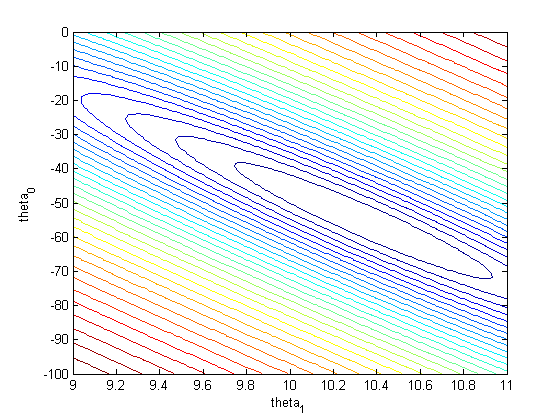
\includegraphics[width=\linewidth/2]{../images/LossContour} 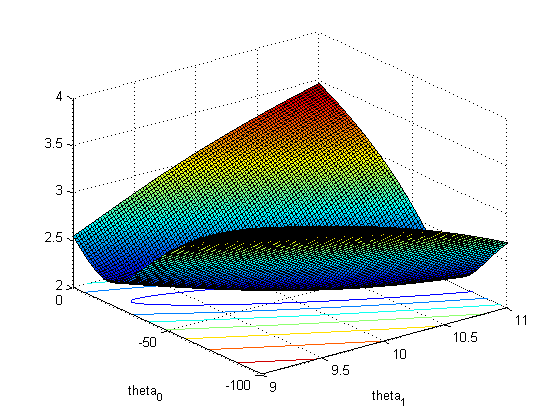
\includegraphics[width=\linewidth/2]{../images/LossSurface}\\
 
 \bigskip
 
\begin{lstlisting}   
function [theta0_vals, theta1_vals, J] = lossfctn( x, y, theta0range, theta1range )
    theta0_vals = zeros(1,100);
    theta1_vals = zeros(1,100);
    theta0s = theta0range(1):(theta0range(2) - theta0range(1))/99:theta0range(2);
    theta1s = theta1range(1):(theta1range(2) - theta1range(1))/99:theta1range(2);
    J = zeros(100);
    numPoints = length(x);
    for i = 1:length(theta0s)
        theta0_vals(i) = theta0s(i);
        for j = 1:length(theta1s)
            theta1_vals(j) = theta1s(j);
            total = 0;
            for n = 1:numPoints
                h = theta0s(i) + theta1s(j)*x(n);
                total = total + (h - y(n))^2;
            end
            total = (0.5/numPoints) * total;
            J(i, j) = total;
        end
    end
end
\end{lstlisting}

\newpage

\item[2.]
	For $\alpha = 2$ after 42,687 iterations the algorithm converged at $\theta_0 = -55.1441$ and $\theta_1 = 10.3370$\\
	For $\alpha = 3$ the algorithm times out after 50,000 iterations with \texttt{NaN} for $\theta_0$ and  $\theta_1$ because the step size was too large. This led to it being unstable and diverging.\\
	
	Polyfit results were $\theta_0 = -55.1756$ and $\theta_1 = 10.3381$\\
	
	Both sets of values are close to the visual estimate of  $\theta_0$ and  $\theta_1$ from \texttt{(1c)}\\
	
	Left: Best fit line (magenta) overlaid on \texttt{ac} and \texttt{gawks} data (blue).\\
	Right: Contour plot displaying progression of $\theta_0$ and  $\theta_1$\\
	
	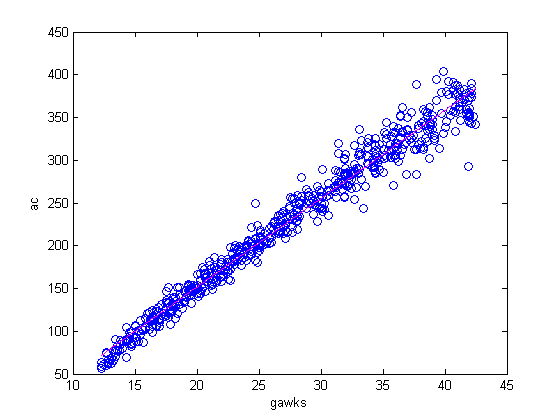
\includegraphics[width=\linewidth/2]{../images/GradientDescent} 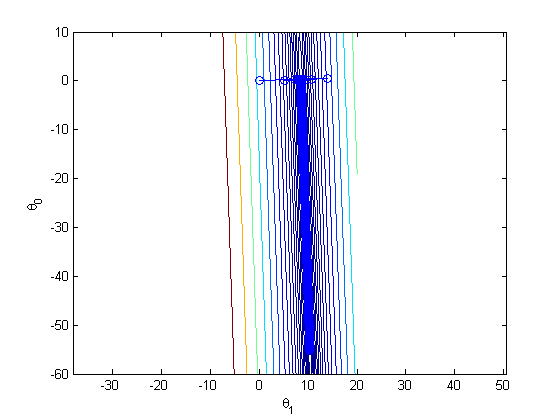
\includegraphics[width=\linewidth/2]{../images/GradientContour}\\

\bigskip

\begin{lstlisting}   
function theta = gradientdescent( x, y, alpha, theta_init, tol )
    maxIters = 50000;
    iter = 0;
    numPoints = length(x);
    theta0 = theta_init(1);
    theta1 = theta_init(2);
    theta = [theta0 theta1];
    while iter < maxIters
        iter = iter + 1;
        theta0Total = 0;
        theta1Total = 0;
        for i = 1:numPoints
            h = theta0 + theta1 * x(i);
            theta0Total = theta0Total + (h - y(i));
            theta1Total = theta1Total + (h - y(i)) * x(i);
        end
        theta0_old = theta0;
        theta1_old = theta1;
        theta0 = theta0 - alpha / numPoints * theta0Total;
        theta1 = theta1 - alpha / numPoints * theta1Total;
        theta = [theta; theta0 theta1];
        theta0Check = abs((theta0 - theta0_old) / theta0_old);
        theta1Check = abs((theta1 - theta1_old) / theta1_old);
        if theta0Check < tol && theta1Check < tol, break, end
    end
end
\end{lstlisting}

\newpage

\item[3.]
	For the \texttt{ac} and \texttt{gawks} data $CI(1) = 3.922$ and $CI(2) = 0.137$\\

\bigskip

\begin{lstlisting}   
function CI = confidenceintervals(x, y, theta)
    theta0 = theta(1);
    theta1 = theta(2);
    numPoints = length(x);
    totalSE = 0;
    for n = 1:numPoints
        h = theta0 + theta1*x(n);
        totalSE = totalSE + (h - y(n))^2;
    end
    SEres = sqrt(totalSE / (numPoints - 2));
    D = numPoints * sum(x.^2) - sum(x)^2;
    SETheta0 = SEres * sqrt(sum(x.^2) / D);
    SETheta1 = SEres * sqrt(numPoints / D);
    CI = [1.96*SETheta0 1.96*SETheta1];
end
\end{lstlisting}

\newpage

\item[4.]
	\texttt{i\_start} = 594\\
	\texttt{i\_exp} = 994\\
	\texttt{t(i\_start)} = 5.93\\
	\texttt{t(i\_exp)} = 9.93\\
	
	Maximum step size before instability is $\alpha = 1.5$, which results in $\theta_0 = -55.175$ and $\theta_1 = 10.338$\\

	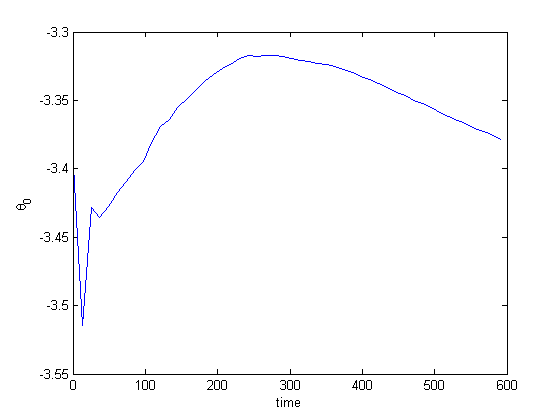
\includegraphics[width=\linewidth/2]{../images/TvecTheta0} 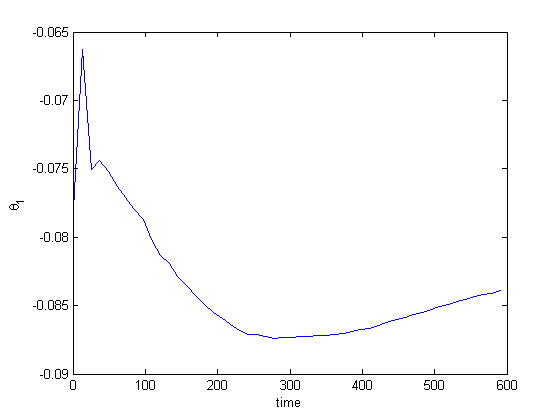
\includegraphics[width=\linewidth/2]{../images/TvecTheta1}\\

\bigskip

\begin{lstlisting}   
function [ theta0, theta1, ci ] = glucosepredict( t, I )
    
    x_norm = (t - min(t))/(max(t)-min(t));
    y_norm = (I - min(I))/(max(I)-min(I));

    descentLog = gradientdescent(x_norm, y_norm, 0.01, [0 0], 1e-4);
    temp = descentLog(end, :);
    theta0Prime = temp(1);
    theta1Prime = temp(2);

    theta0 = min(I) + theta0Prime * (max(I) - min(I)) - theta1Prime * min(t) * ((max(I) - min(I)) / (max(t) - min(t)));
    theta1 = theta1Prime * ((max(I) - min(I)) / (max(t) - min(t)));

    ci = confidenceintervals(t, I, [theta0 theta1]);
end


\end{lstlisting}
\end{enumerate}

\end{document}